\documentclass{standalone}
\usepackage{graphicx}
\usepackage{siunitx}
\usepackage{tikz} % To generate the plot from csv
\usepackage{varwidth}
\usepackage[normalem]{ulem}
\usetikzlibrary{shapes,arrows}
\usetikzlibrary{backgrounds}
\usetikzlibrary{matrix, positioning, fit}
\usetikzlibrary{patterns}
\definecolor{forestgreen}{rgb}{0.0, 0.5, 0.0}
\usetikzlibrary{decorations.pathreplacing}
\tikzstyle{smallcircle} =[fill=black!100, text=white, circle, inner sep=1pt, minimum size=0.1em]
\tikzstyle{ourcircle} = [draw, semicircle, inner sep=0pt,minimum size=2pt]
\tikzstyle{dullblock} = [draw, fill=black!20, circle, minimum height=2em, minimum width=2em]
\tikzstyle{block} = [draw=black, rounded corners, thick, line width=0.3mm, rectangle, minimum height=10em, minimum width=7em]
\tikzstyle{blocksmall} = [draw=black, thick, line width=0.5mm, rectangle, minimum height=6em, minimum width=3em, fill=white]
\tikzstyle{group} = [draw=black, line width=0.3mm, rectangle, minimum height=2em, minimum width=2em]
\tikzstyle{textblock} = [draw, fill=black!20, rectangle, rounded corners]
\tikzstyle{rectblock} = [draw, rectangle, minimum height=1.3em]
\tikzstyle{plain} = []
\tikzstyle{decisionblock} = [draw, diamond, fill=black!20]
\tikzstyle{input} = [draw, thick, fill=blue!20, circle, minimum size=1pt]
\tikzstyle{output} = [draw, fill=blue!20, circle, minimum size=1pt]
\tikzstyle{pinstyle} = [pin edge={to-,thin,black}]
\tikzset{toprule/.style={%
        execute at end cell={%
            \draw [line cap=rect,#1] (\tikzmatrixname-\the\pgfmatrixcurrentrow-\the\pgfmatrixcurrentcolumn.north west) -- (\tikzmatrixname-\the\pgfmatrixcurrentrow-\the\pgfmatrixcurrentcolumn.north east);%
        }
    },
    bottomrule/.style={%
        execute at end cell={%
            \draw [line cap=rect,#1] (\tikzmatrixname-\the\pgfmatrixcurrentrow-\the\pgfmatrixcurrentcolumn.south west) -- (\tikzmatrixname-\the\pgfmatrixcurrentrow-\the\pgfmatrixcurrentcolumn.south east);%
        }
    }
}

\begin{document}

    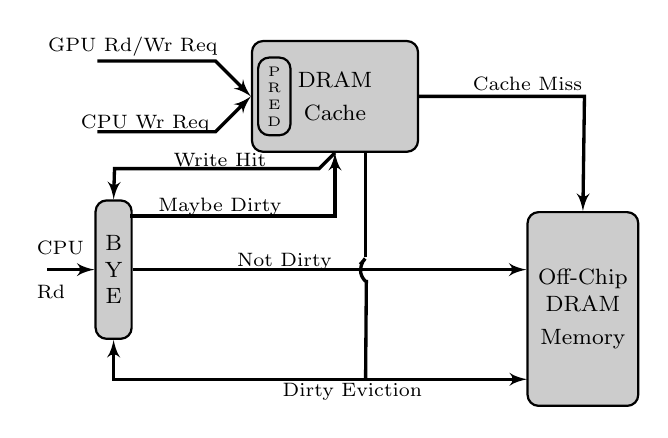
\begin{tikzpicture}[auto, >=latex']
        % Blocks
        \node [textblock, thick, minimum height=5em] (bye){\begin{varwidth}{4cm} \centering{\footnotesize{B\\Y\\E\\}} \end{varwidth}};
        \node [textblock, thick, minimum width=6em, minimum height=4em, right = 1.5cm of bye, yshift=2.2cm] (dramcache){\begin{varwidth}{4cm} \centering{\footnotesize{DRAM\\Cache}} \end{varwidth}};
        \node [textblock, thick, left = 0.01cm of dramcache, xshift=1.5em] (pred){\begin{varwidth}{4cm} \centering{\tiny{P\\R\\E\\D\\}} \end{varwidth}};
        \node [textblock, thick, minimum width=4em, right = 5cm of bye, minimum height=7em, yshift=-0.5cm] (dram){\begin{varwidth}{4cm} \centering{\footnotesize{Off-Chip\\DRAM\\Memory}} \end{varwidth}};

        % Arrows
        \draw [<-,very thick] (bye.west) to [out=180,in=0] ++(-0.6,0);
        \draw [->, very thick] (dramcache.east) to [out=0,in=180] ++(2.1,0) to (dram.north);
        \draw [->, very thick] (dramcache.south) to ++(-0.2,-0.2) to [out=180,in=0] ++(-2.6,0) to (bye.north);
        \draw [<-, very thick] (dramcache.south) to [out=-90,in=90] ++(0,-0.8) to [out=180,in=0] ++(-2.6,0);
        \draw [<->, very thick] (bye.south) to [out=-90,in=90] ++(0,-0.5) to [out=0,in=180] ++(5.25,0);
        \draw [->, very thick] (bye.east) to [out=0,in=180] ++(5,0);
        \draw [<-, very thick] (dramcache.west) to ++(-0.45,0.45) to ++(-1.5,0);
        \draw [<-, very thick] (dramcache.west) to ++(-0.45,-0.45) to ++(-1.5,0);
        \draw [-, very thick, xshift=3.2cm] (0,1.5) to (0,0.16);
        \draw [-, very thick, xshift=3.2cm, right=90, looseness=3] (-0.07,0.067) to (0,-0.15);
        \draw [-, very thick, xshift=3.2cm] (0.01,-0.13) to (0,-1.4);

        % labels
        \node [plain, left=0.01cm of bye, minimum height=1em, minimum width=1em] (cpurd) {\begin{varwidth}{4cm}\scriptsize{CPU\\ \\Rd}\end{varwidth}};
        \node [plain, above=1.4cm of dram, minimum height=1em, minimum width=1em, xshift=-2em] (cachemiss) {\begin{varwidth}{4cm}\scriptsize{Cache Miss}\end{varwidth}};
        \node [plain, left=1.2cm of dram, minimum height=1em, minimum width=1em, yshift=-3em] (dirtyevict) {\begin{varwidth}{4cm}\scriptsize{Dirty Eviction}\end{varwidth}};
        \node [plain, left=0.4cm of dramcache, minimum height=1em, minimum width=1em, yshift=-1em] (WrReq) {\begin{varwidth}{4cm}\scriptsize{CPU Wr Req}\end{varwidth}};
        \node [plain, left=0.3cm of dramcache, minimum height=1em, minimum width=1em, yshift=1.8em] (GpuReq) {\begin{varwidth}{4cm}\scriptsize{GPU Rd/Wr Req}\end{varwidth}};
        \node [plain, right=0.2cm of bye, minimum height=1em, minimum width=1em, yshift=0.8cm] (maydir) {\begin{varwidth}{4cm}\scriptsize{Maybe Dirty}\end{varwidth}};
        \node [plain, right=0.2cm of bye, minimum height=1em, minimum width=1em, yshift=0.1cm, xshift=1cm] (notdir) {\begin{varwidth}{4cm}\scriptsize{Not Dirty}\end{varwidth}};
        \node [plain, above=0.15cm of maydir, minimum height=1em, minimum width=1em] (wrhit) {\begin{varwidth}{4cm}\scriptsize{Write Hit}\end{varwidth}};


    \end{tikzpicture}
\end{document}
